\section{Identifikationd der Reaktionsprodukte mithilfe von LC-MS}

Die Produkte der Reaktion mit Essigsäureanhydrid konnten ebenfalls mithilfe von \gls{lcms} identifiziert werden. In Abbildung 

\begin{figure}[!htbp]
  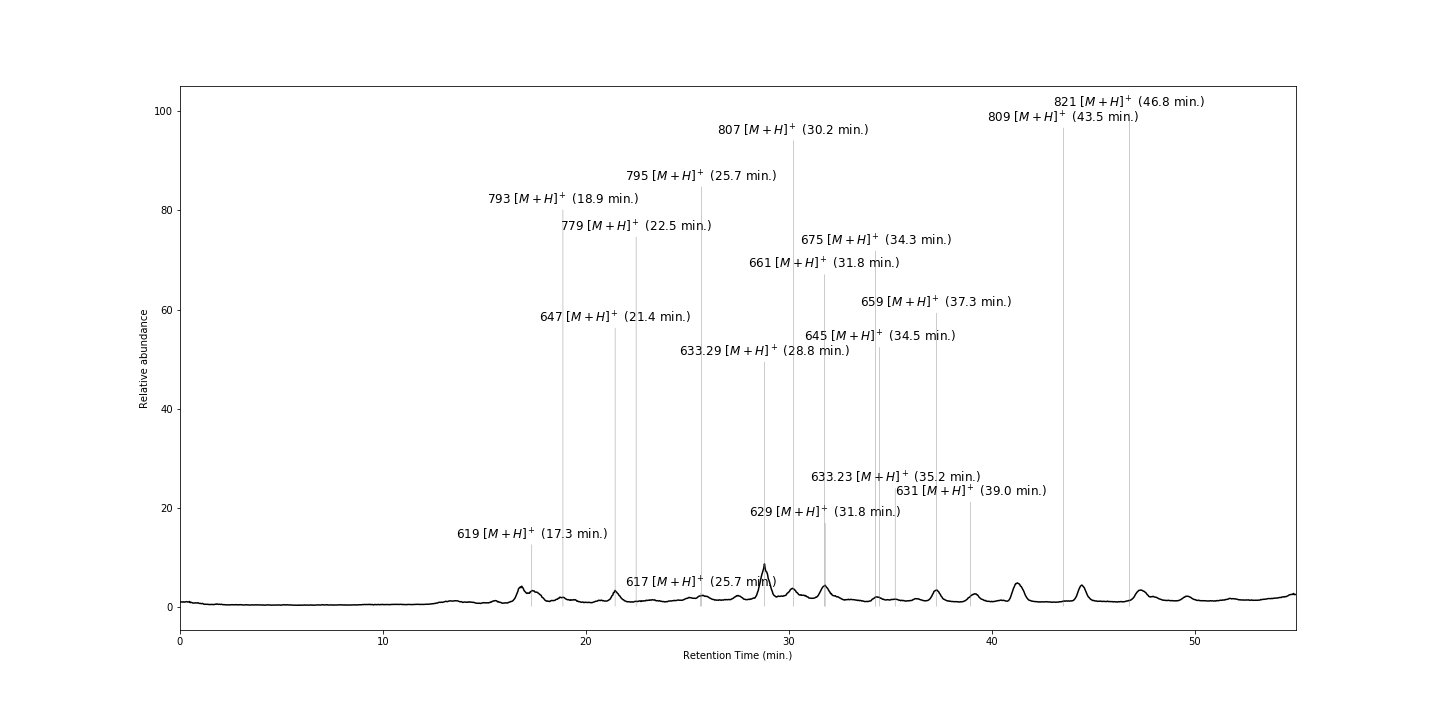
\includegraphics[width=\textwidth]{figures/Kapitel6/Reaktion3h/Kuerbis_Analyse_Reaktion3h_Ganzes_Spektrum.png}
  \caption[LC-MS Chromatogramm nach 3h Reaktionsdauer, Quelle: Author]{\gls{lcms} Chromatogramm}
  \label{fig:LCMSCChromatogrammRP}
\end{figure}


\begin{figure}[!htbp]
  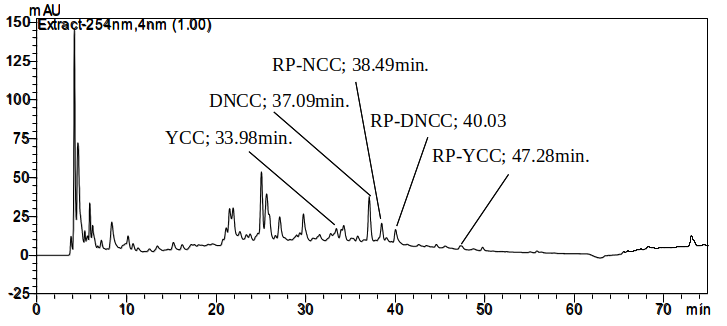
\includegraphics[width=\textwidth]{figures/Kapitel6/Reaktion3h/HPLC_Chromatogramm.png}
  \caption[HPLC Chromatogramm nach 3h Reaktionsdauer, Quelle: Author]{\gls{hplc} Chromatogramm}
  \label{fig:HPLCChromatogrammRP}
\end{figure}

\begin{figure}[!htbp]
  \begin{subfigure}[b]{0.5\textwidth}
    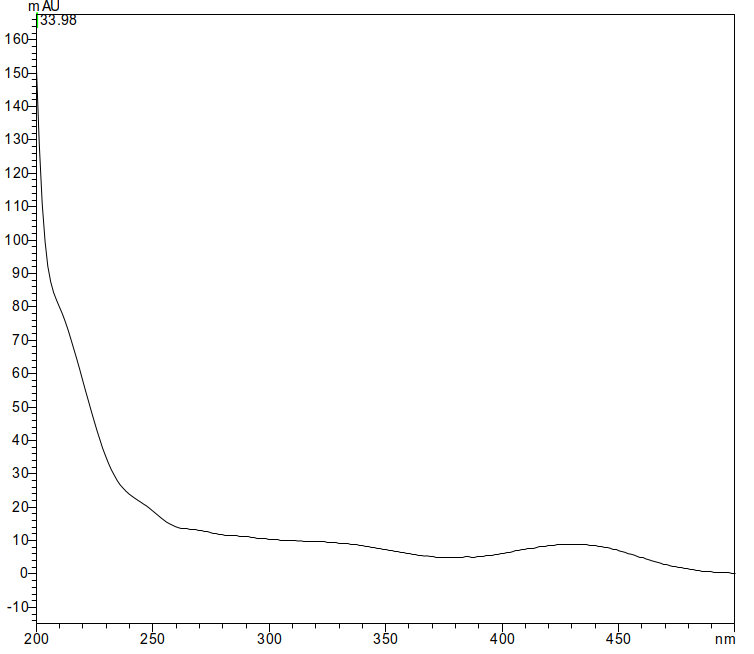
\includegraphics[width=\textwidth]{figures/Kapitel6/Reaktion3h/YCC3398.png}
    \caption{}
    \label{fig:YCC3398}
  \end{subfigure}
  \hfill
  \begin{subfigure}[b]{0.5\textwidth}
    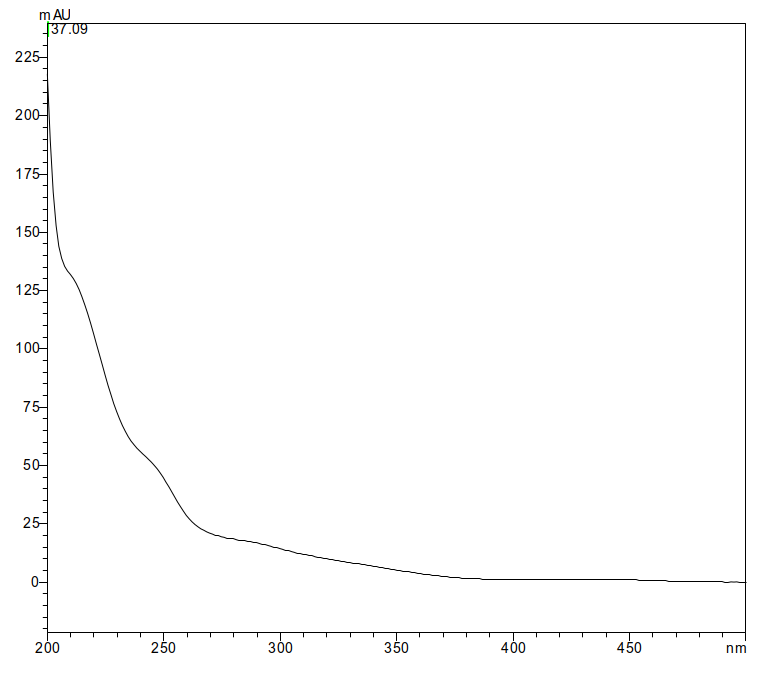
\includegraphics[width=\textwidth]{figures/Kapitel6/Reaktion3h/DNCC3709.png}
    \caption{}
    \label{fig:DNCC3709}
  \end{subfigure}
  
  \begin{subfigure}[b]{0.5\textwidth}
    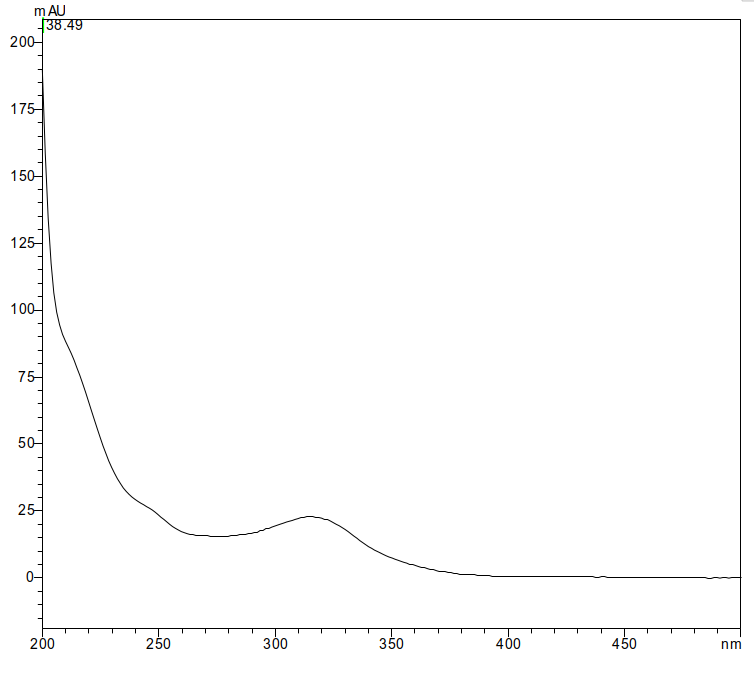
\includegraphics[width=\textwidth]{figures/Kapitel6/Reaktion3h/NCC3849.png}
    \caption{}
    \label{fig:NCC3849}
  \end{subfigure}
  \hfill
  \begin{subfigure}[b]{0.5\textwidth}
    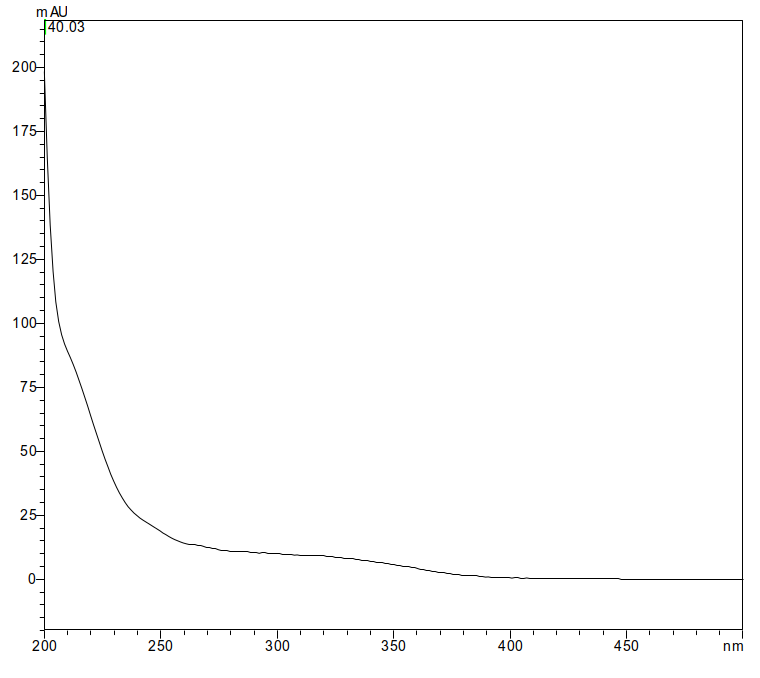
\includegraphics[width=\textwidth]{figures/Kapitel6/Reaktion3h/DNCC4003.png}
    \caption{}
    \label{fig:DNCC4003}
  \end{subfigure}
  
  \begin{subfigure}[b]{0.5\textwidth}
    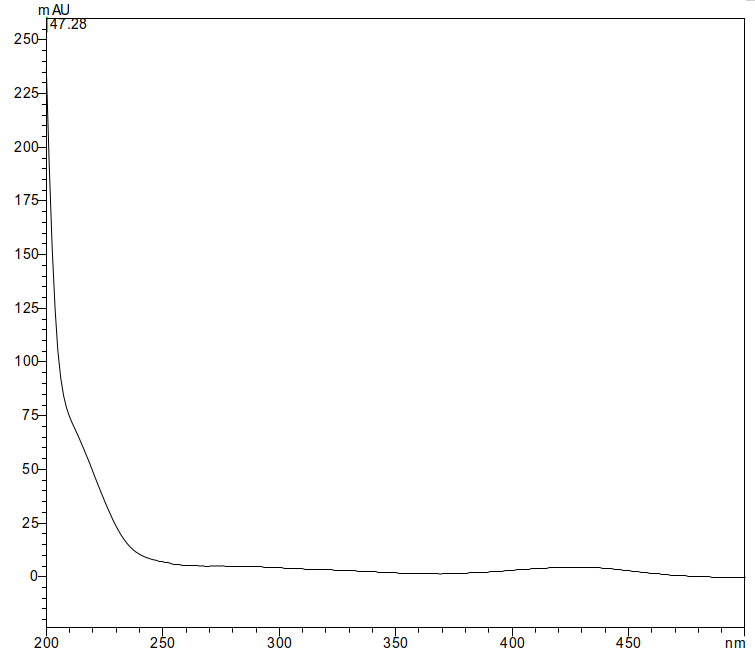
\includegraphics[width=\textwidth]{figures/Kapitel6/Reaktion3h/YCC4728.png}
    \caption{}
    \label{fig:YCC4728}
  \end{subfigure}
  \caption[UV/Vis online Spektren mit der Charakteristik eines YCC bei 33.98min., eines DNCC bei 37.09min. eines NCC bei 38.94min., eines DNCC bei 40.03min. sowie eines YCC bei 47.28min., Quelle: Author]{UV/Vis online Spektren: charakeristisch für (a) \gls{YCC} - RT = 33.98min., (b) \gls{DNCC} - RT = 37.09min., (c) \gls{NCC} - RT = 38.94min., (d) \gls{DNCC} - RT = 40.03min., (e) \gls{YCC} - RT = 47.28min.}
\end{figure}

